\chapter[Methods for amino acid-level predictions]{Hyperdimensional computing methods for\\amino acid-level\\predictions}
\section{Introduction}
As discussed in section~\ref{ssec:nlp}, state-of-the-art protein language models primarily rely on transformer-based architectures to learn representations of protein sequences and amino acids in the context of other amino acids. These models have demonstrated their effectiveness in various applications, such as protein function prediction and protein-protein interaction prediction, by capturing complex patterns in amino acid sequences. Moreover, these models are also capable of making detailed predictions at the amino acid level, such as predicting secondary structure. This involves determining local three-dimensional structures of regions within a protein, such as alpha-helices and beta-sheets, based on the sequence of amino acids. This capability further extends their utility in understanding protein structure and function. However, these models are computationally intensive and may be less suitable for certain tasks or scenarios where computational resources are limited.

In section~\ref{sssec:trans}, we explored the idea of encoding information from a residue's neighborhood into a hyperdimensional vector that represents the residue and its surroundings. This approach allows us to capture local sequence information and can serve as an effective encoding scheme for amino acids. To evaluate the effectiveness of this encoding method, we will employ it as an input for several perceptron-based models.

Perceptron-based models, a type of artificial neural network model, have been employed for various machine learning tasks over the years, including classification and regression problems. The perceptron, one of the simplest and earliest types of neural networks, was proposed by Frank Rosenblatt in 1958~\cite{perceptron}. A perceptron consists of a single artificial neuron that receives multiple input features and computes a weighted sum of these inputs. This weighted sum is then passed through an activation function, which determines the output of the perceptron. The learning process involves adjusting the weights of the input features iteratively, using a rule that minimizes prediction errors on the training data. The perceptron learning algorithm starts with an initial set of weights, typically set to zero or small random values. For each instance in the training data, the perceptron computes the output, compares it with the true label, and updates the weights accordingly. The weight update rule is based on the difference between the predicted output and the true label, multiplied by the learning rate and the input feature value. Single-layer perceptrons consist of an input layer and an output layer of perceptrons, allowing for multiclass classifications. However, they can only solve linearly separable problems, limiting their applicability for more complex tasks.

As single-layer perceptrons can only solve linearly separable problems, researchers developed more complex neural network architectures, such as multi-layer perceptrons (MLP), which consist of multiple layers of artificial neurons connected in a feedforward manner. MLPs can learn non-linear patterns in the data by using non-linear activation functions (e.g., sigmoid, tanh, ReLU) and employing backpropagation for weight updates~\cite{mlp}. This enhanced ability to model non-linear relationships allows MLPs to tackle a wider range of problems.

By combining the residue neighborhood encoding method with perceptron-based models, we could develop more computationally efficient alternatives to state-of-the-art transformer-based models. These models may provide valuable insights into protein sequences and amino acids while being more suitable for scenarios with limited computational resources. 

The aim of this chapter is to design and implement a simple perceptron-based neural network that utilizes hyperdimensional vectors of residues in a protein sequence as inputs. The goal is to train the network to discern and learn the secondary structure of these residues based on their surrounding counterparts. Ultimately, this should enable our model to accurately and efficiently predict the secondary structures of residues in protein sequences whose structure is unknown.

\section{Methods}
We built straightforward perceptron-based neural networks that take as input a hyperdimensional vector, in particular a neighborhood-encoded amino acid vector made as described in section~\ref{sssec:trans}. It should then output the amino acid's secondary structure, either 3- or 8-state as shown in figure~\cite{fig:pipe2}.

\begin{figure}[H]
    \centering
    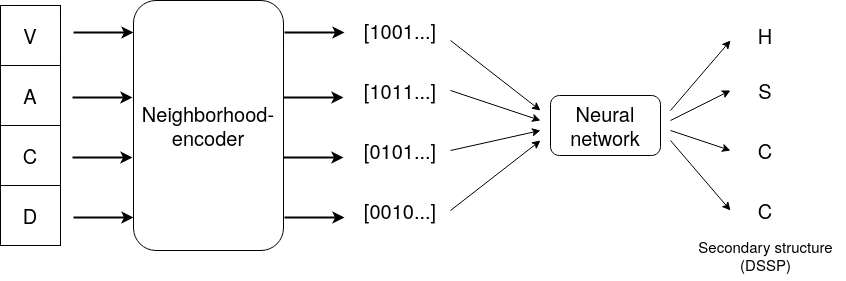
\includegraphics[scale = 0.43]{pipeline2}
    \caption{A simple demonstration of our pipeline to classify amino acids on their secondary structure based on their neighborhood-encoded vectors. First, a residue is encoded by neighborhood-encoding as discussed in section~\ref{sssec:trans}. Then, this vector is used as an input for a trained neural network to predict its secondary structure state. This is done for every residue in every given protein sequence.}\label{fig:pipe2}
\end{figure}

We used the training dataset compiled by Klausen \textit{et al.} for their model protein language model NetsurfP 2.0~\cite{netsurf} as our training dataset. It contains 10,337 protein sequences obtained from the Protein Data Bank (PDB)~\cite{pdb}. Each residue in these sequences is annotated with its 3- and 8-class secondary structure classification according to \textit{Define Secondary Structure of Proteins} (DSSP)~\cite{dssp}, providing a comprehensive description of the protein's structural properties. All residues have been encoded using our neighborhood-encoder as described in section~\ref{sec:trans} with $n=25$ and $n=100$ using random hyperdimensional vectors for each amino acid. Due to computational memory constraints, we randomly selected 60 \% of the sequences from the original dataset for training and testing (80 \% and 20 \% respectively), ensuring a representative sample of the data.

In summary, we have four distinct supervised training sets. The first model is trained on neighborhood-encodings of range $n=25$ with a 3-state secondary level. The second model also uses neighborhood-encodings of range $n=25$, but with an 8-state secondary level. The third model is trained on neighborhood-encodings of range $n=100$, using a 3-state secondary level. Finally, the fourth model uses neighborhood-encodings of range $n=100$ and an 8-state secondary level.

As for the perceptron-based methods, to decrease the computational time, we opted to build, train and evaluate the model in Python due to its support for computations on GPUs on our systems. We employed PyTorch-Lightning v1.8.4 for model construction and training and CUDA v11.7.0 on a high-performance computing (HPC) cluster equipped with an NVIDIA V100 GPU. The model comprised fully-connected layers with an input layer size equal to the dimension of the hyperdimensional vectors (10,000 in this case). Depending on the secondary structure classification desired, the output layer size was set to either 3 or 8 depending on the secondary structure classification. We used a batch size of 128 during training. Between each layer, we incorporated a ReLU (Rectified Linear Unit) activation function to introduce non-linearity into the model. The training loss was monitored using cross-entropy loss. To optimize the model, we employed the widely-used ADAM optimizer. We evaluated various configurations and hyperparameters to determine the best-performing but still computationally feasible approach:

\begin{table}[h]
    \caption{Overview of model configurations and hyperparameters tested}
    \label{tab:casp8}
    \centering
    \begin{tabular}{l|ccc}
        \toprule
         & Epochs & Learning rate & Size hidden layer(s)\\
        \midrule
        \textbf{SLP} & 100 & 0.03 & /\\
        \hline
        \textbf{1-layer MLP} & 50 & 0.003 & 500\\
        \hline
        \textbf{10-layer MLP} & 200 & 0.0003 & \makecell{8000-5000-2000-1000-800-\\500-200-100-50-20}\\
        \bottomrule
    \end{tabular}
  \end{table}

As test datasets, we opted to use CB513~\cite{cb513} and CASP12~\cite{casp12} (compiled by the developers of NetSurfP 2.0~\cite{netsurf}) since they are easily attainable and commonly used by researchers as benchmark datasets for protein language models. The MLP model with 10 hidden layers was trained using 60 \% of the training data and then evaluated using these test datasets. For extra validation, random dummy data was generated.

\section{Results}
Figure~\ref{fig:main8} shows the training progress of the SLP-based models. They show notable issues with the SLP models' ability to train effectively on our dataset. This is signaled by the substantial fluctuations in both loss and validation performance, a trend suggesting an inherent instability in the learning process of this model. The 1-layer MLP model also exhibits problematic behavior, as it does not learn as seen in its loss-curves in figure~\ref{fig:main83}. On top of that, it predicts only one single class during validation (the class with the highest proportion), resulting in a large discrepancy between the accuracy and F1-score. All of this could be attributed to the simplicity of these models, which might not have the capacity to capture the complex patterns in the data. These limitations lead to our decision to discontinue further investigations and experimentation with these particular models.

Figure~\ref{fig:main8e} presents the outcome of the training procedure. In contrast to the SLP and the 1-layer MLP models, the performance of the much deeper 10-layer MLP model demonstrates much more stable and consistent behavior throughout the training process, as evidenced by the performance and loss metrics, even though the resulting performance remains generally low. Although this stability may partially result from the lower learning rate, the model's computational feasibility made it an option for further investigation, prompting us to select this 133,343,733-parameter model for our subsequent tests with various datasets and comparisons with other state-of-the-art methods.

\begin{figure}[htbp]
    \centering
    \begin{subfigure}{0.48\textwidth}
        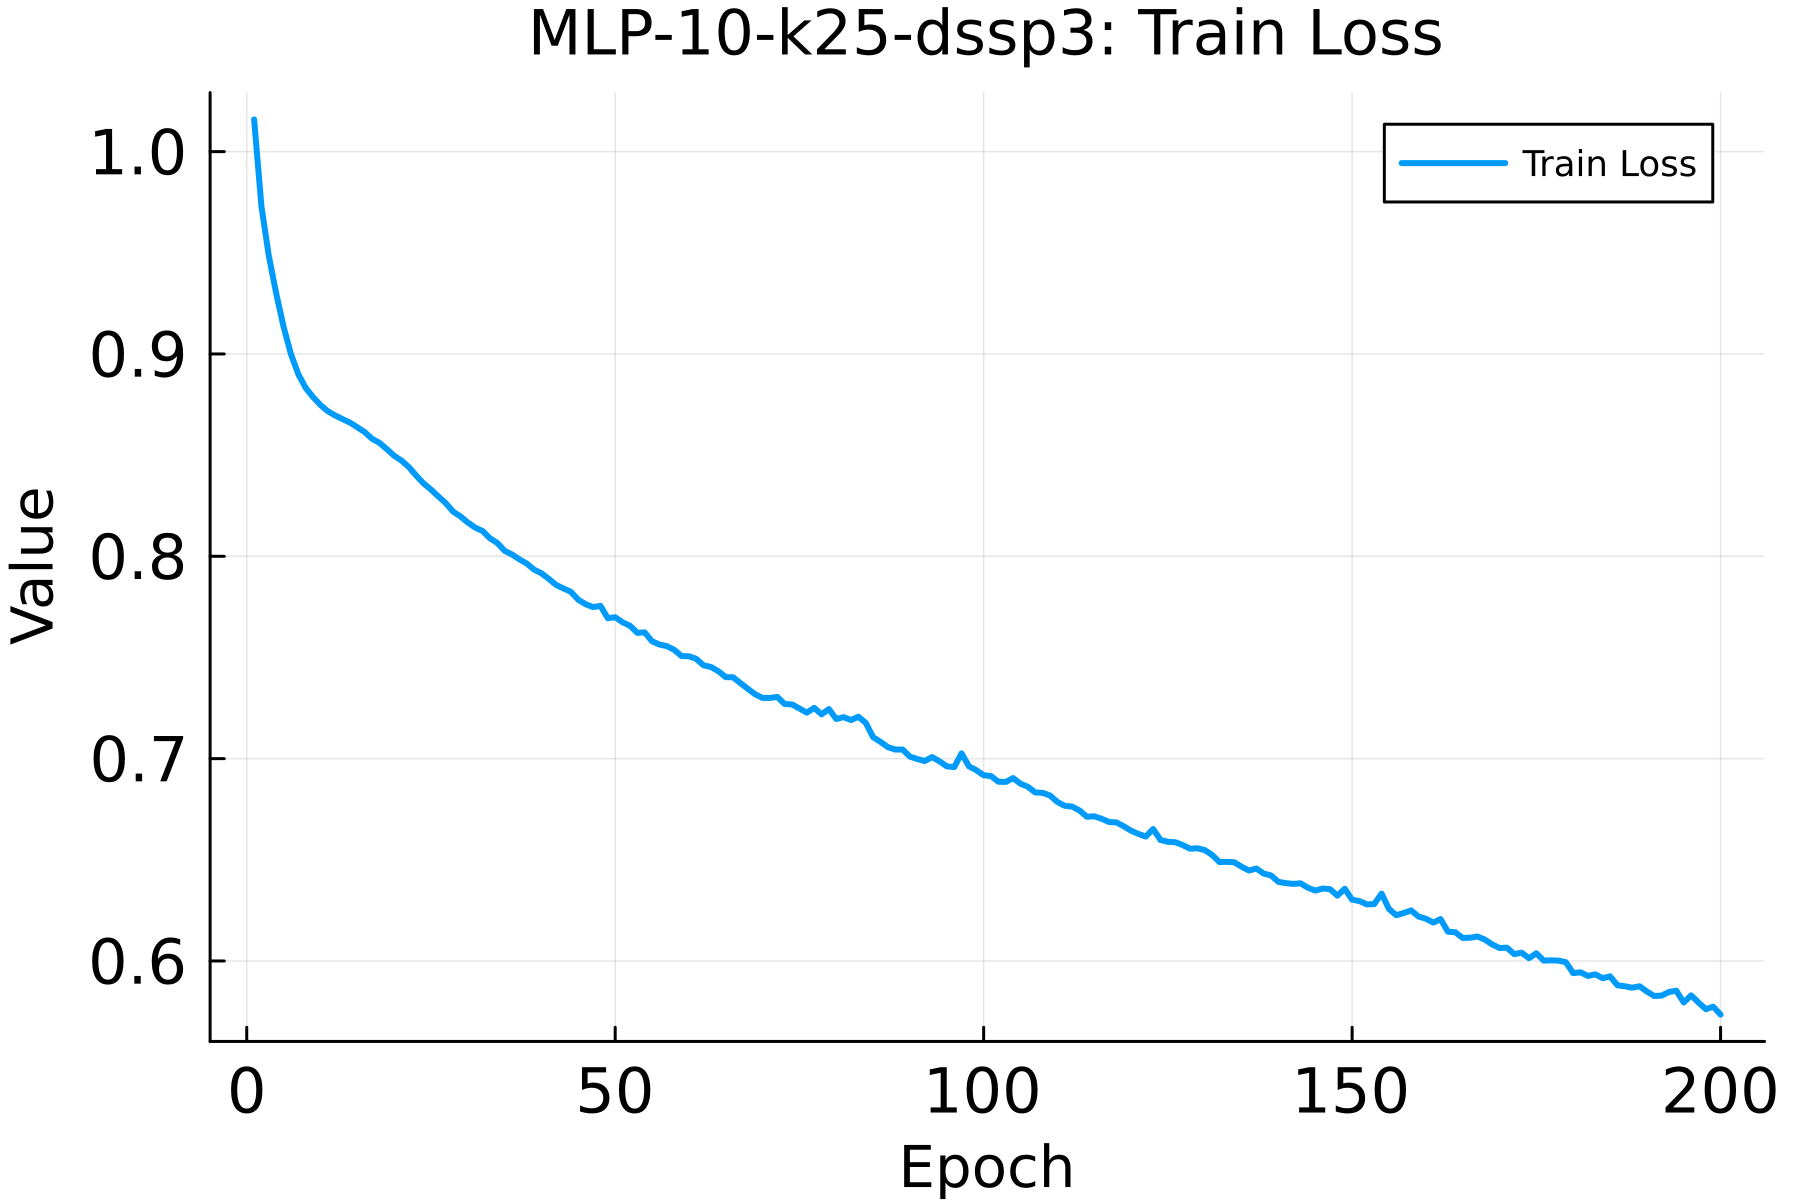
\includegraphics[width=\textwidth]{mlp_fullk25_dssp3_loss}
        \label{fig:subefig}
    \end{subfigure}
    \hfill
    \begin{subfigure}{0.48\textwidth}
        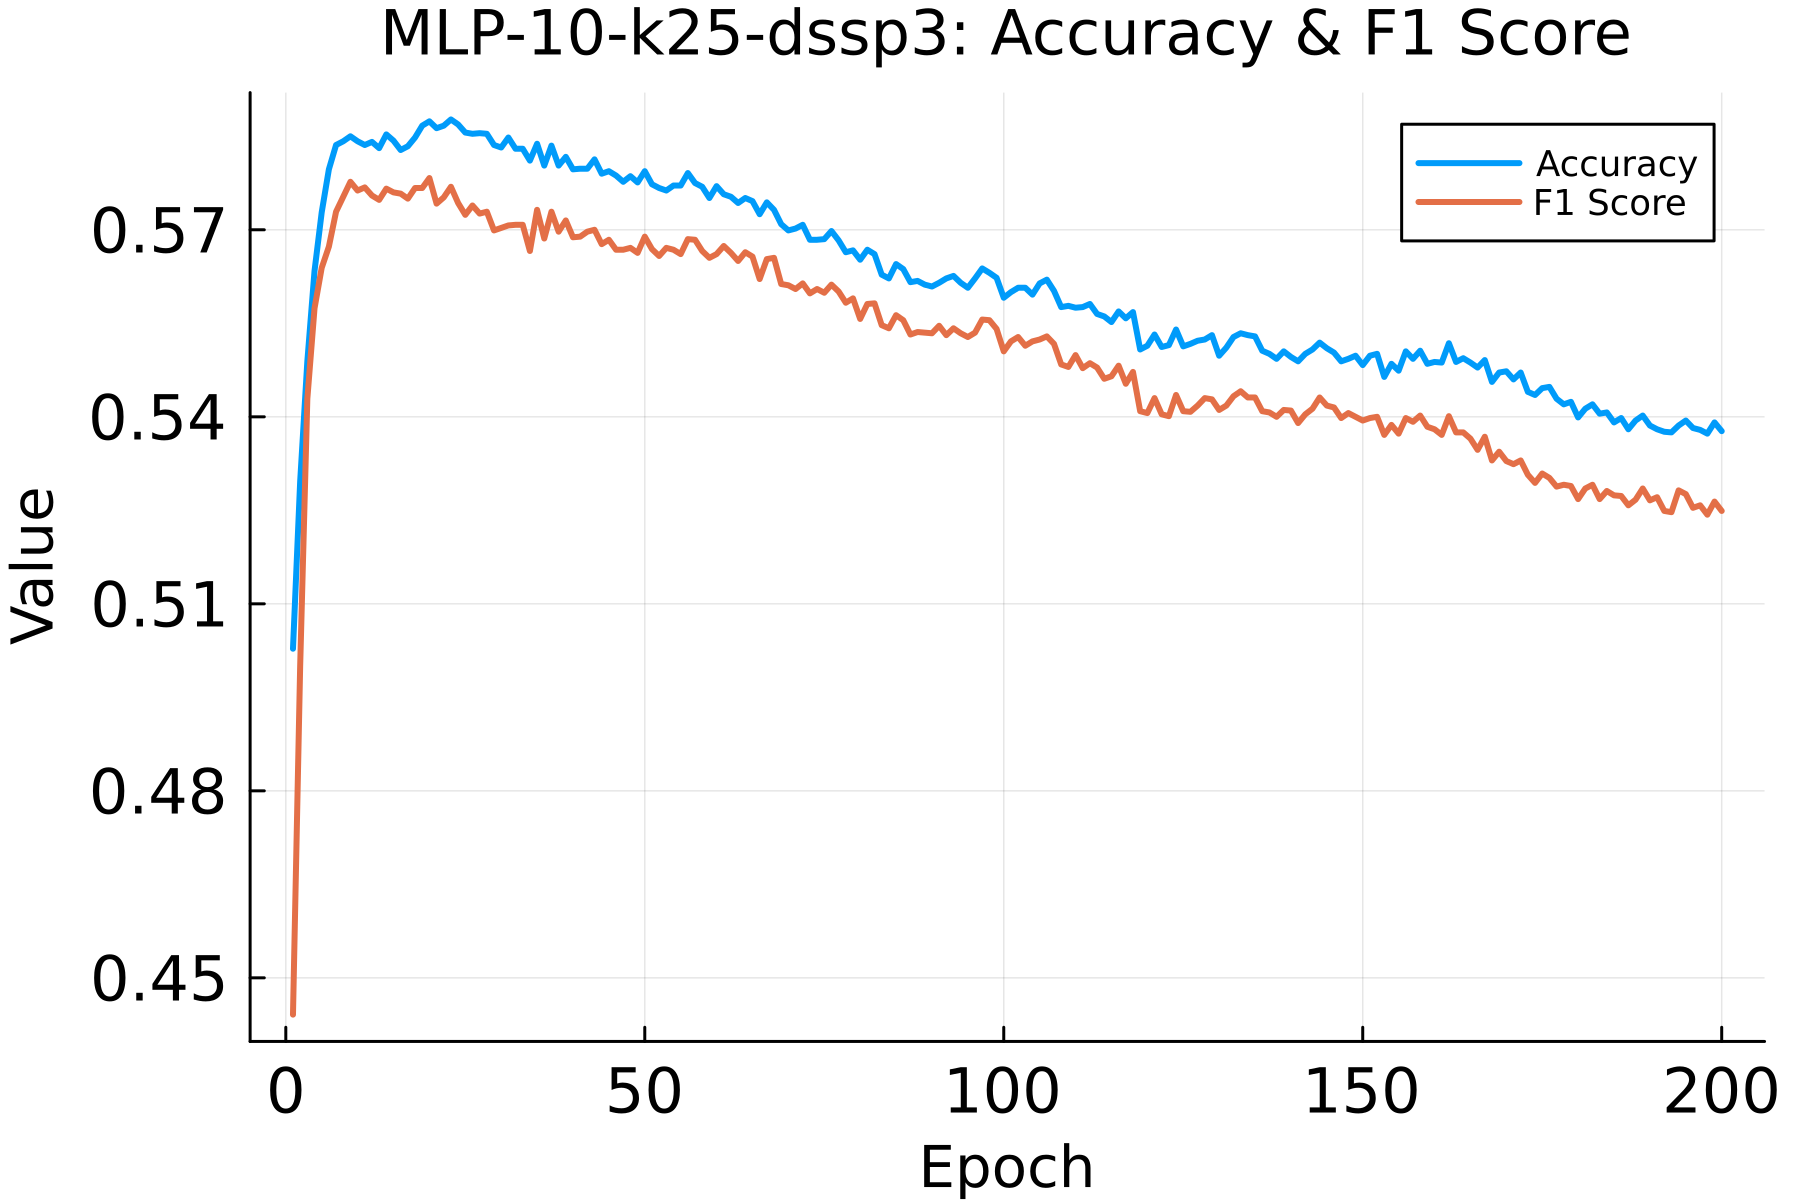
\includegraphics[width=\textwidth]{mlpfull_k25_dssp3_score}
        \label{fig:subefi}
    \end{subfigure}
    
    \begin{subfigure}{0.48\textwidth}
        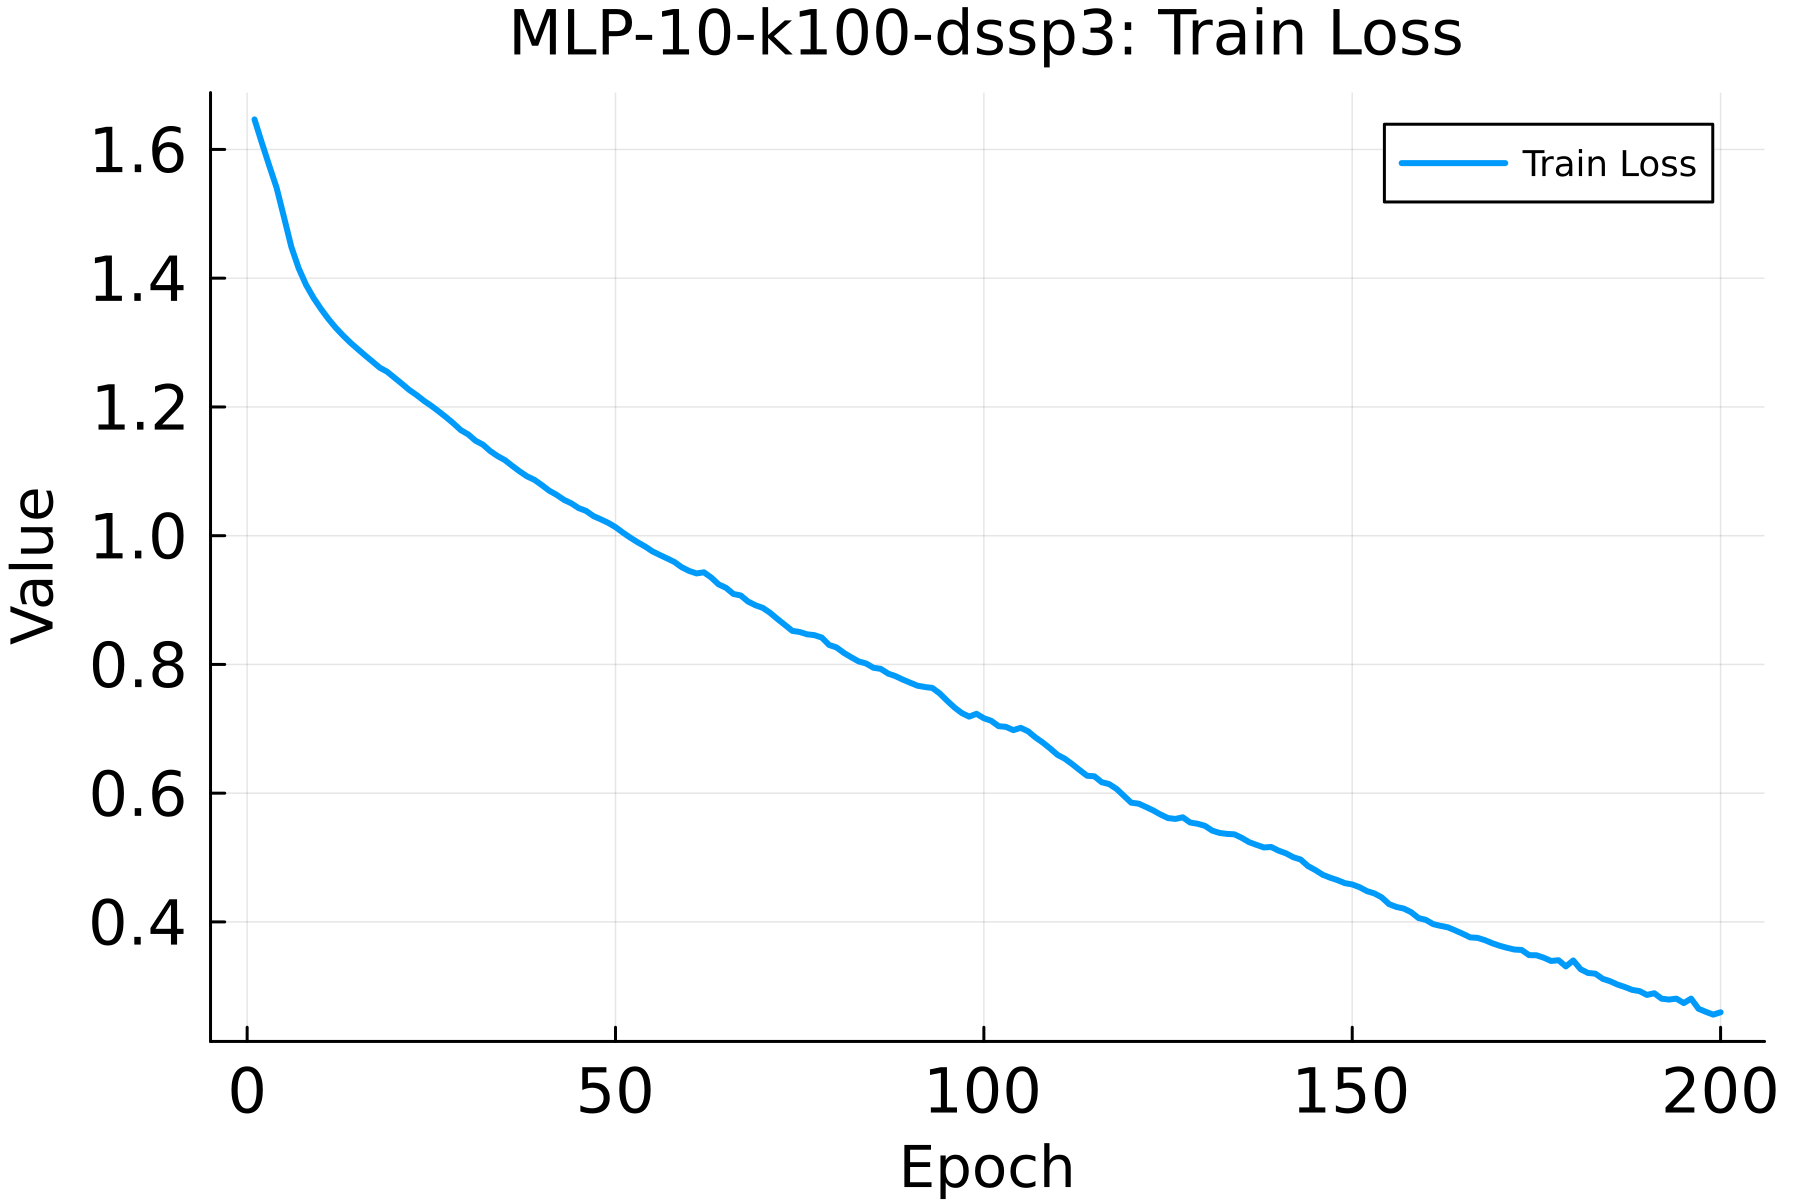
\includegraphics[width=\textwidth]{mlp_fullk25_dssp8_loss}
        \label{fig:subef}
    \end{subfigure}
    \hfill
    \begin{subfigure}{0.48\textwidth}
        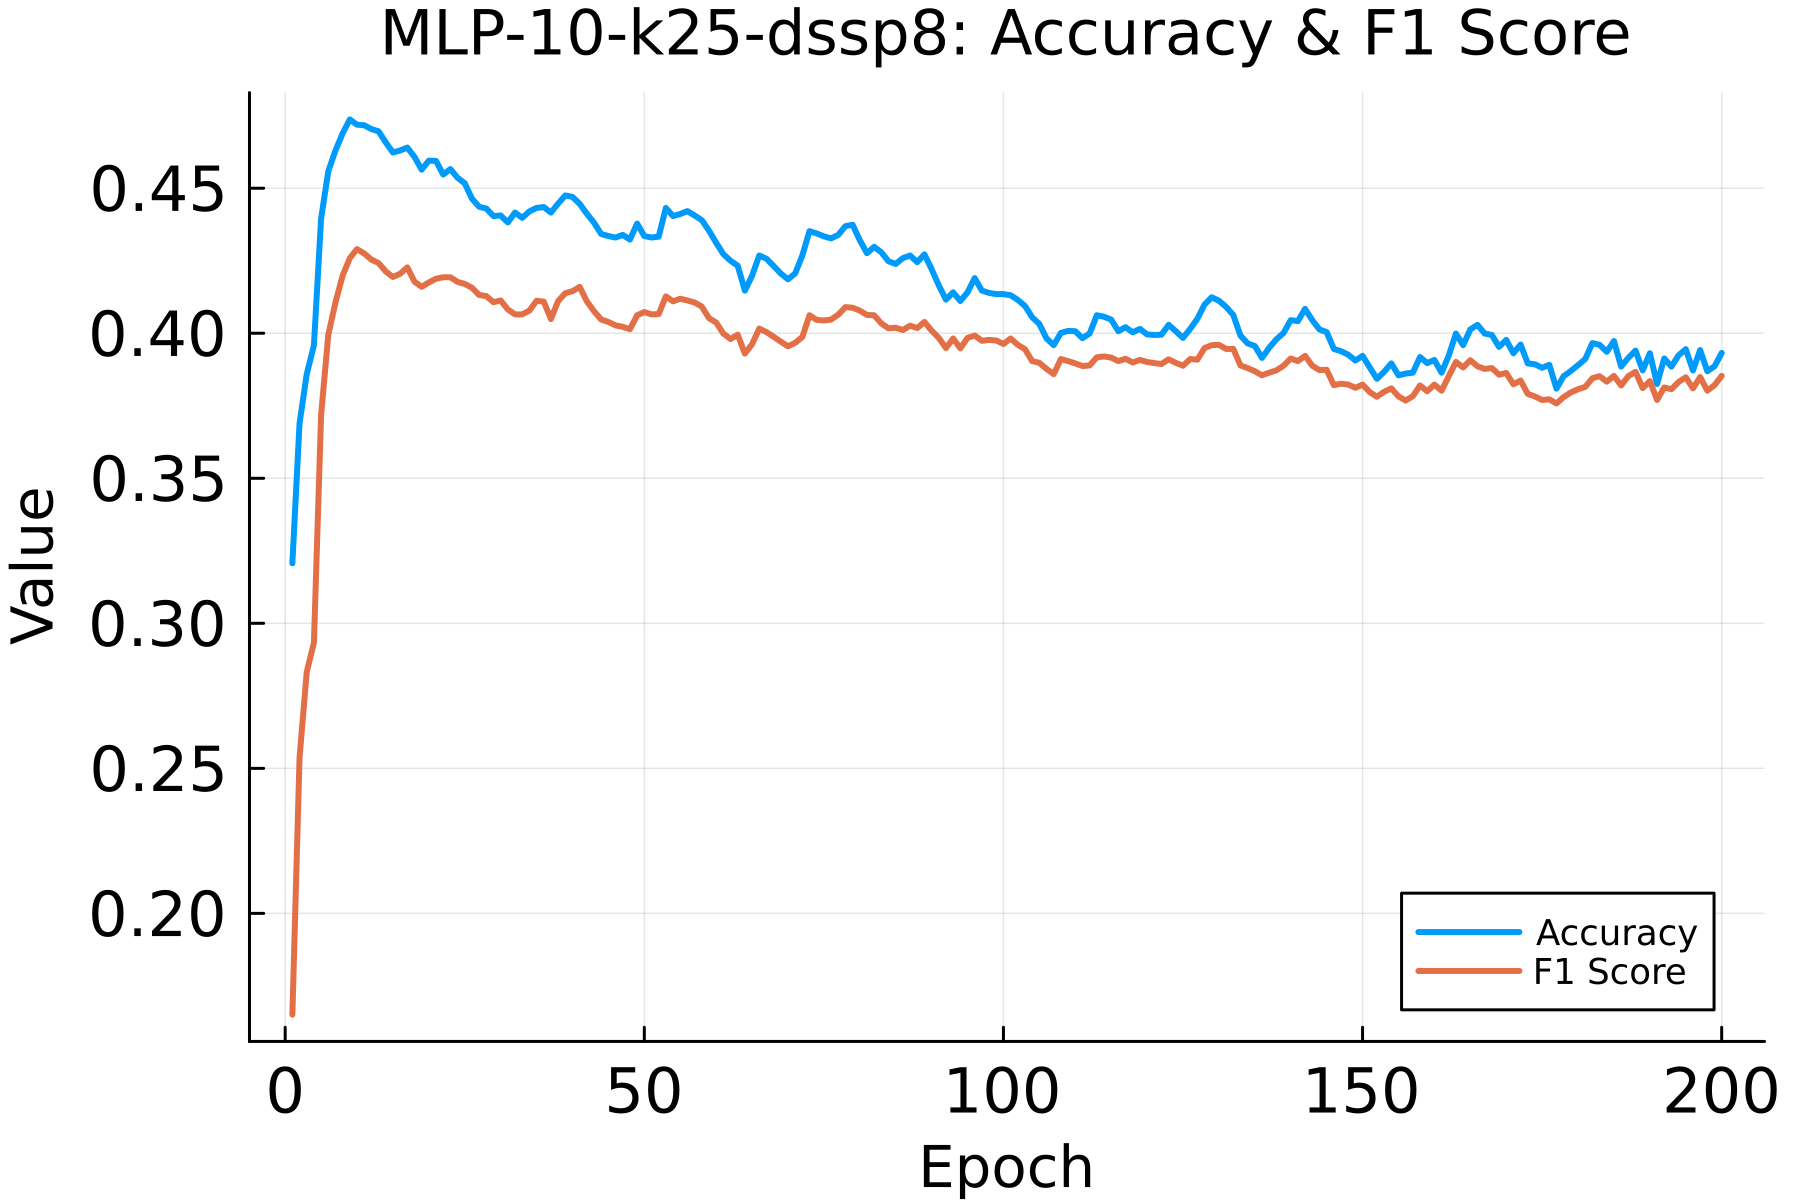
\includegraphics[width=\textwidth]{mlpfull_k25_dssp8_score}
        \label{fig:sube}
    \end{subfigure}
    
    \begin{subfigure}{0.48\textwidth}
        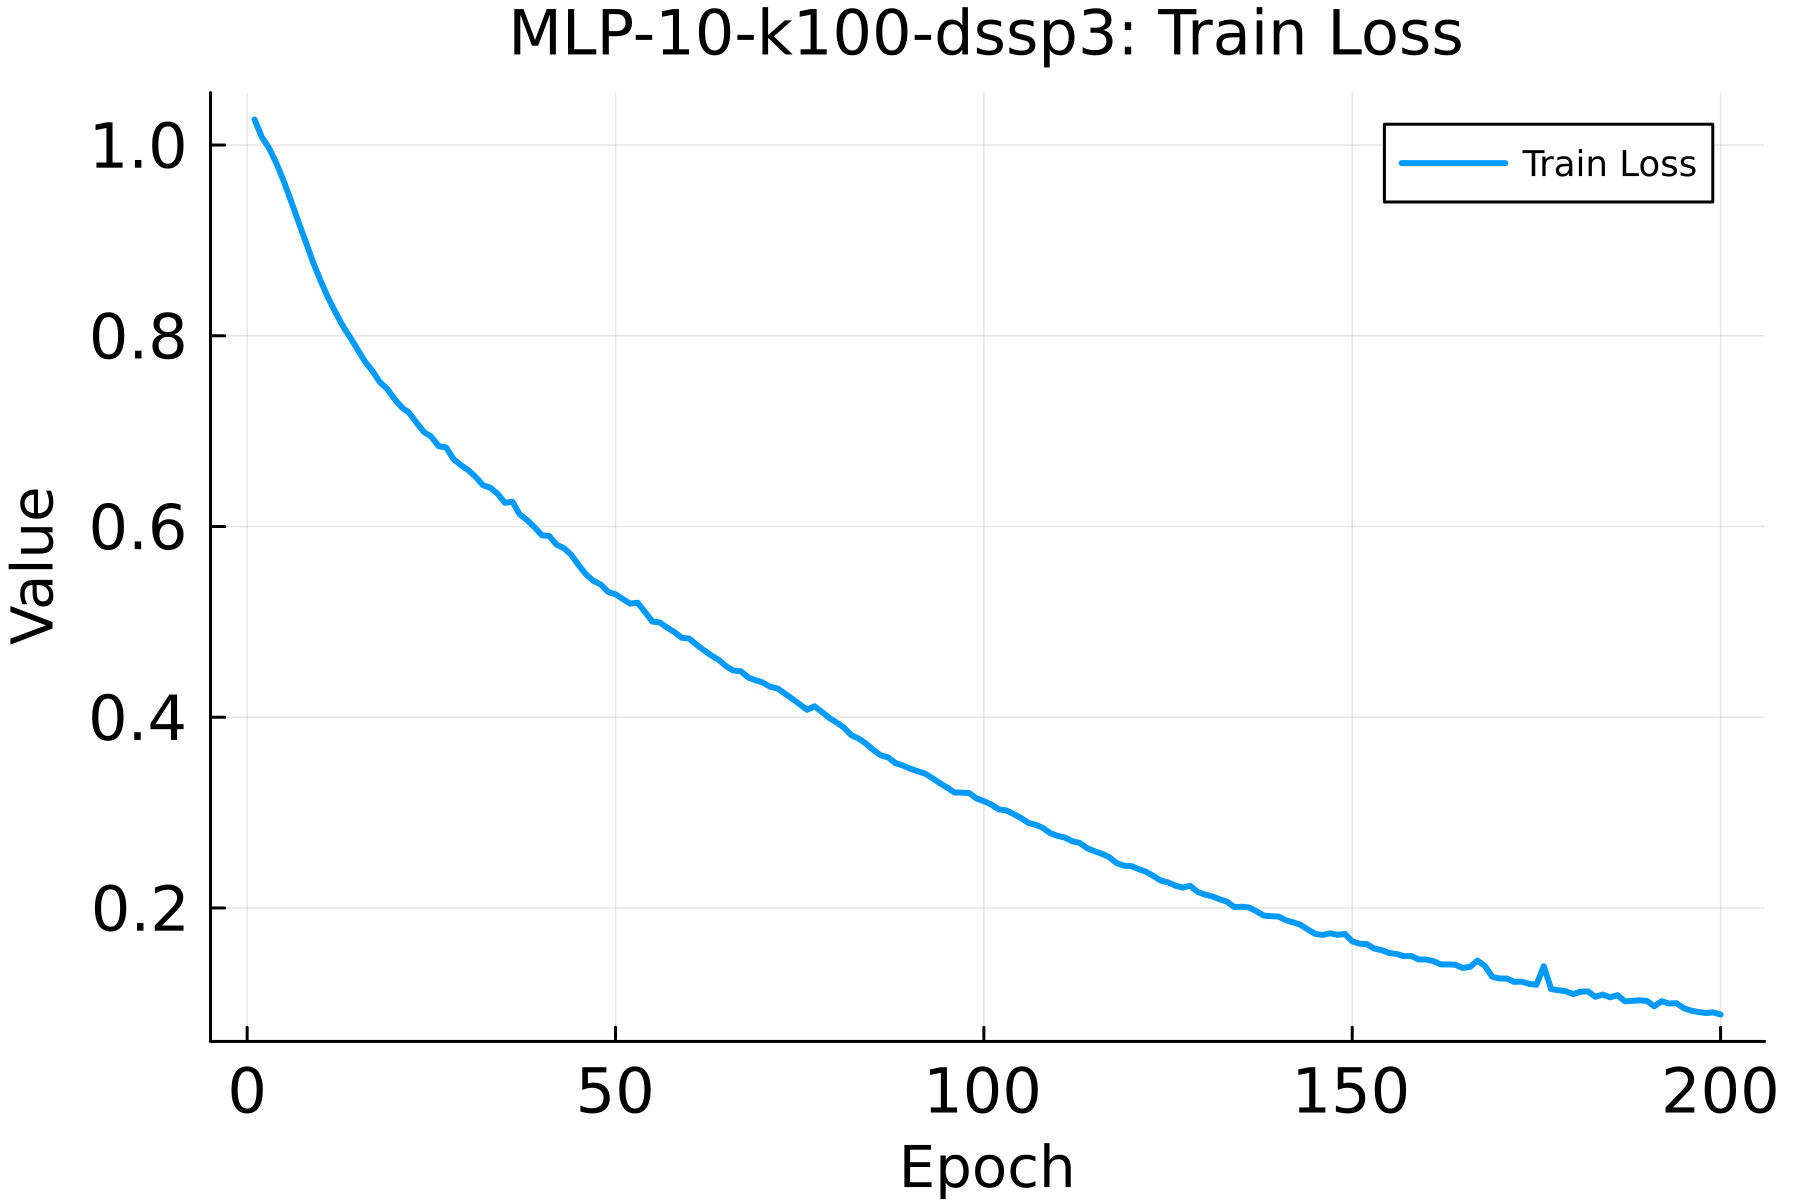
\includegraphics[width=\textwidth]{mlp_fullk100_dssp3_loss}
        \label{fig:sue}
    \end{subfigure}
    \hfill
    \begin{subfigure}{0.48\textwidth}
        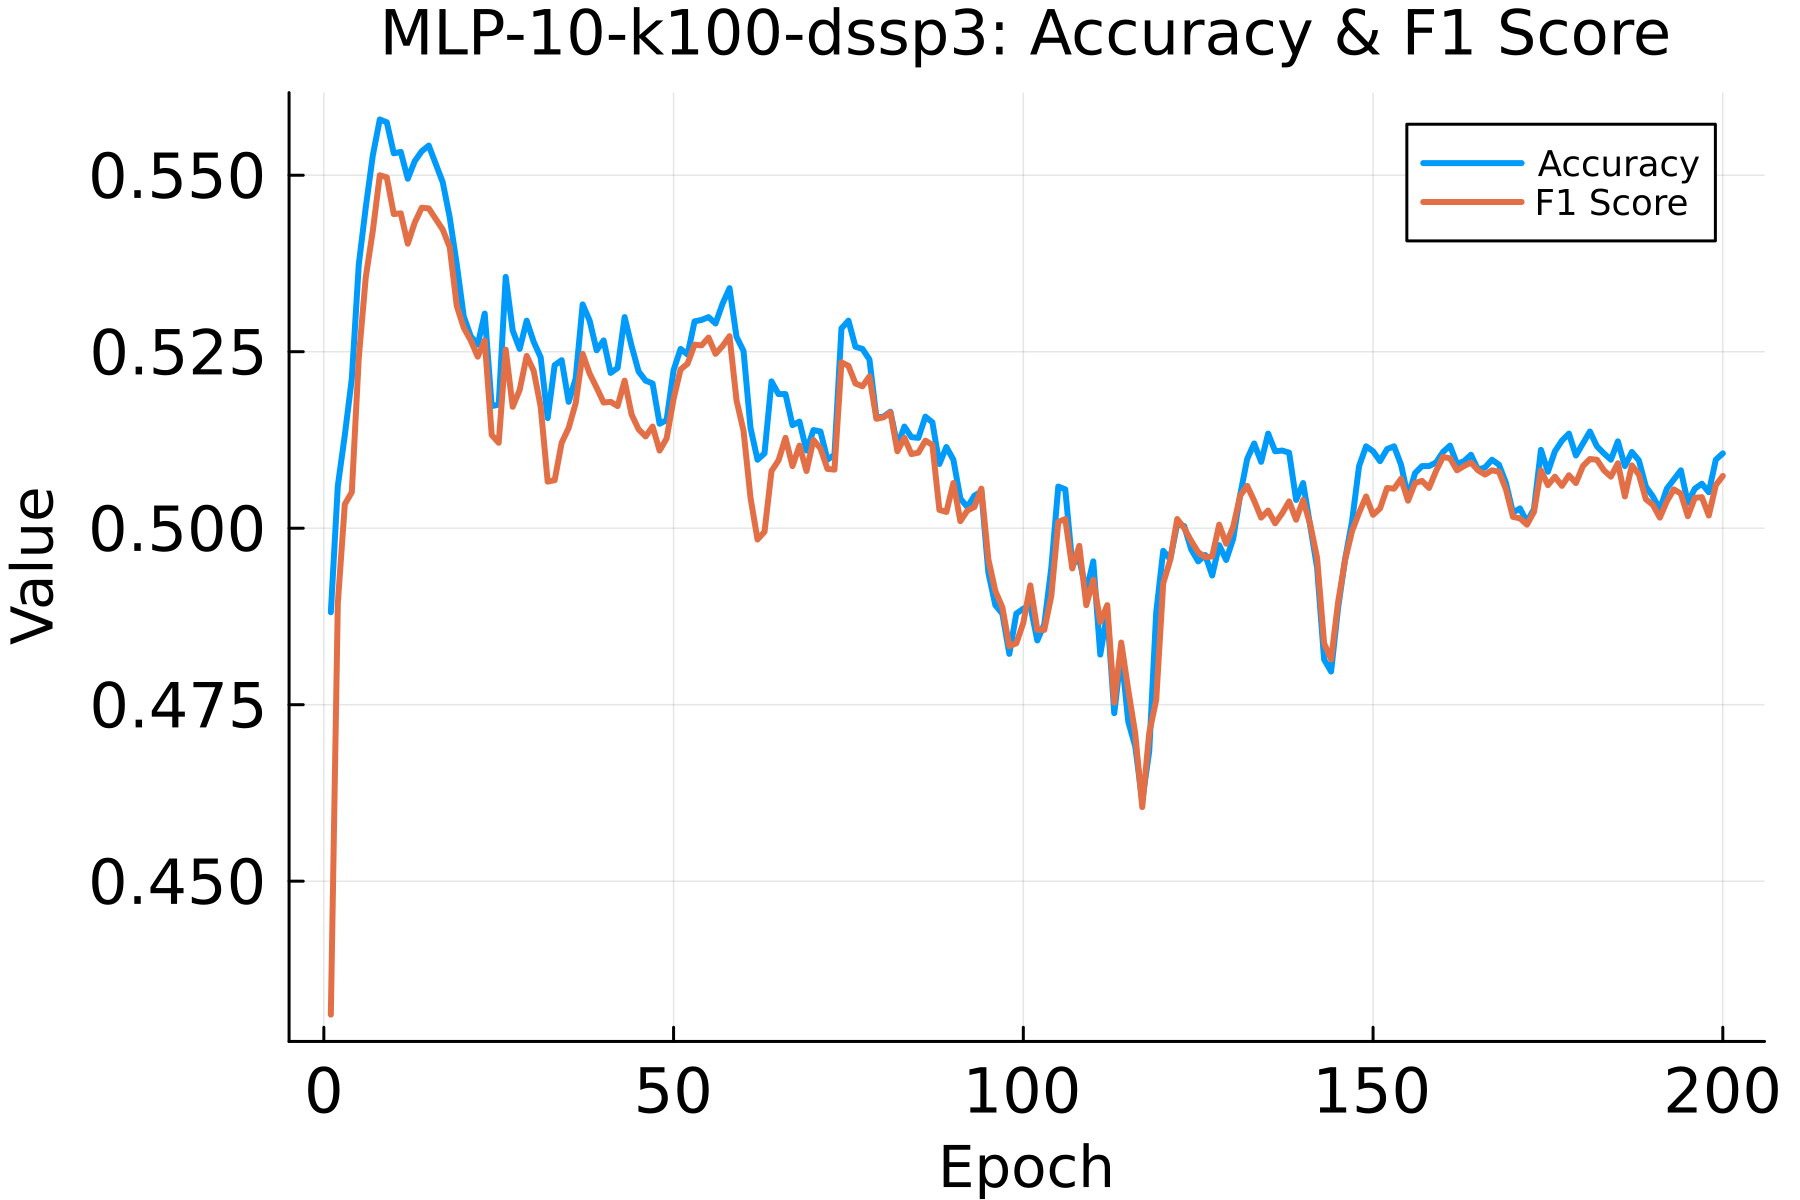
\includegraphics[width=\textwidth]{mlpfull_k100_dssp3_score}
        \label{fig:se}
    \end{subfigure}
    
    \begin{subfigure}{0.48\textwidth}
        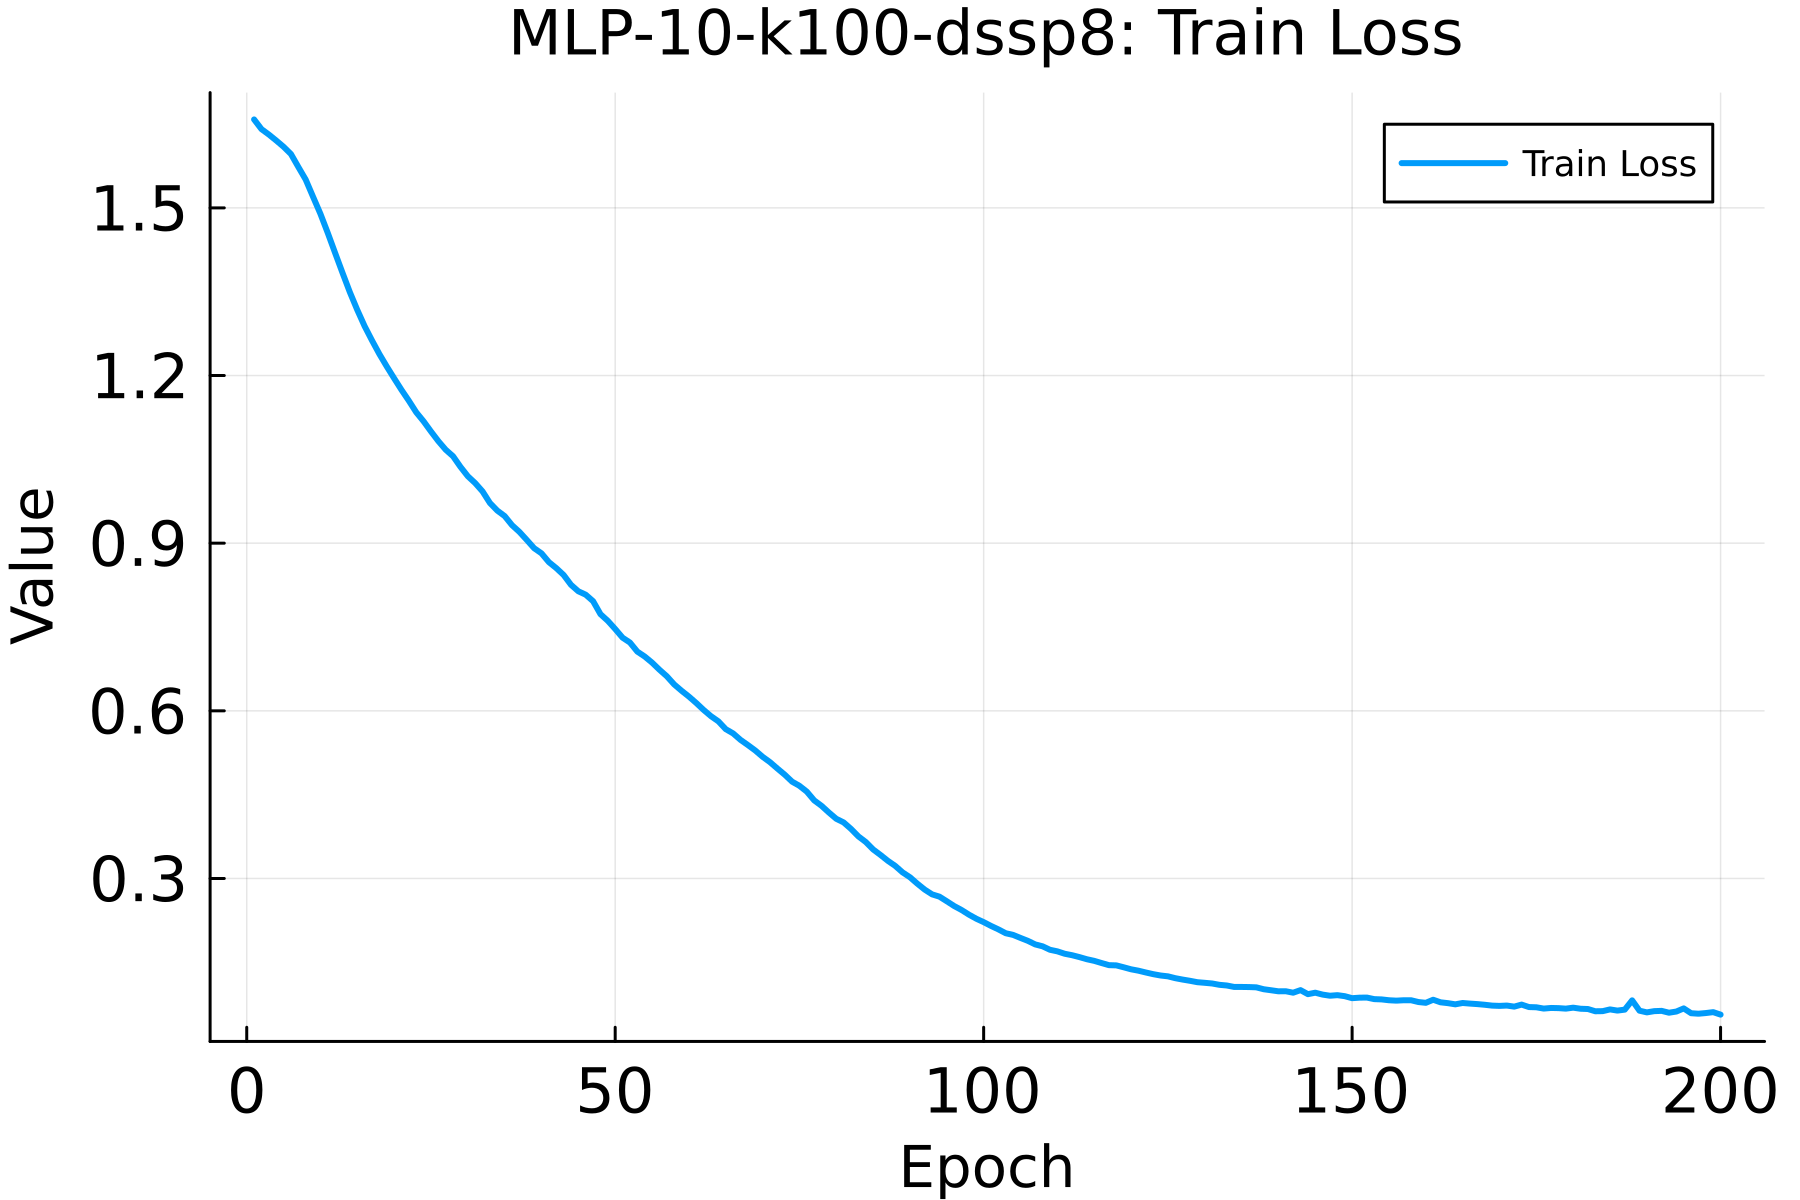
\includegraphics[width=\textwidth]{mlp_full_k100_dssp8_loss}
        \label{fig:sge}
    \end{subfigure}
    \hfill
    \begin{subfigure}{0.48\textwidth}
        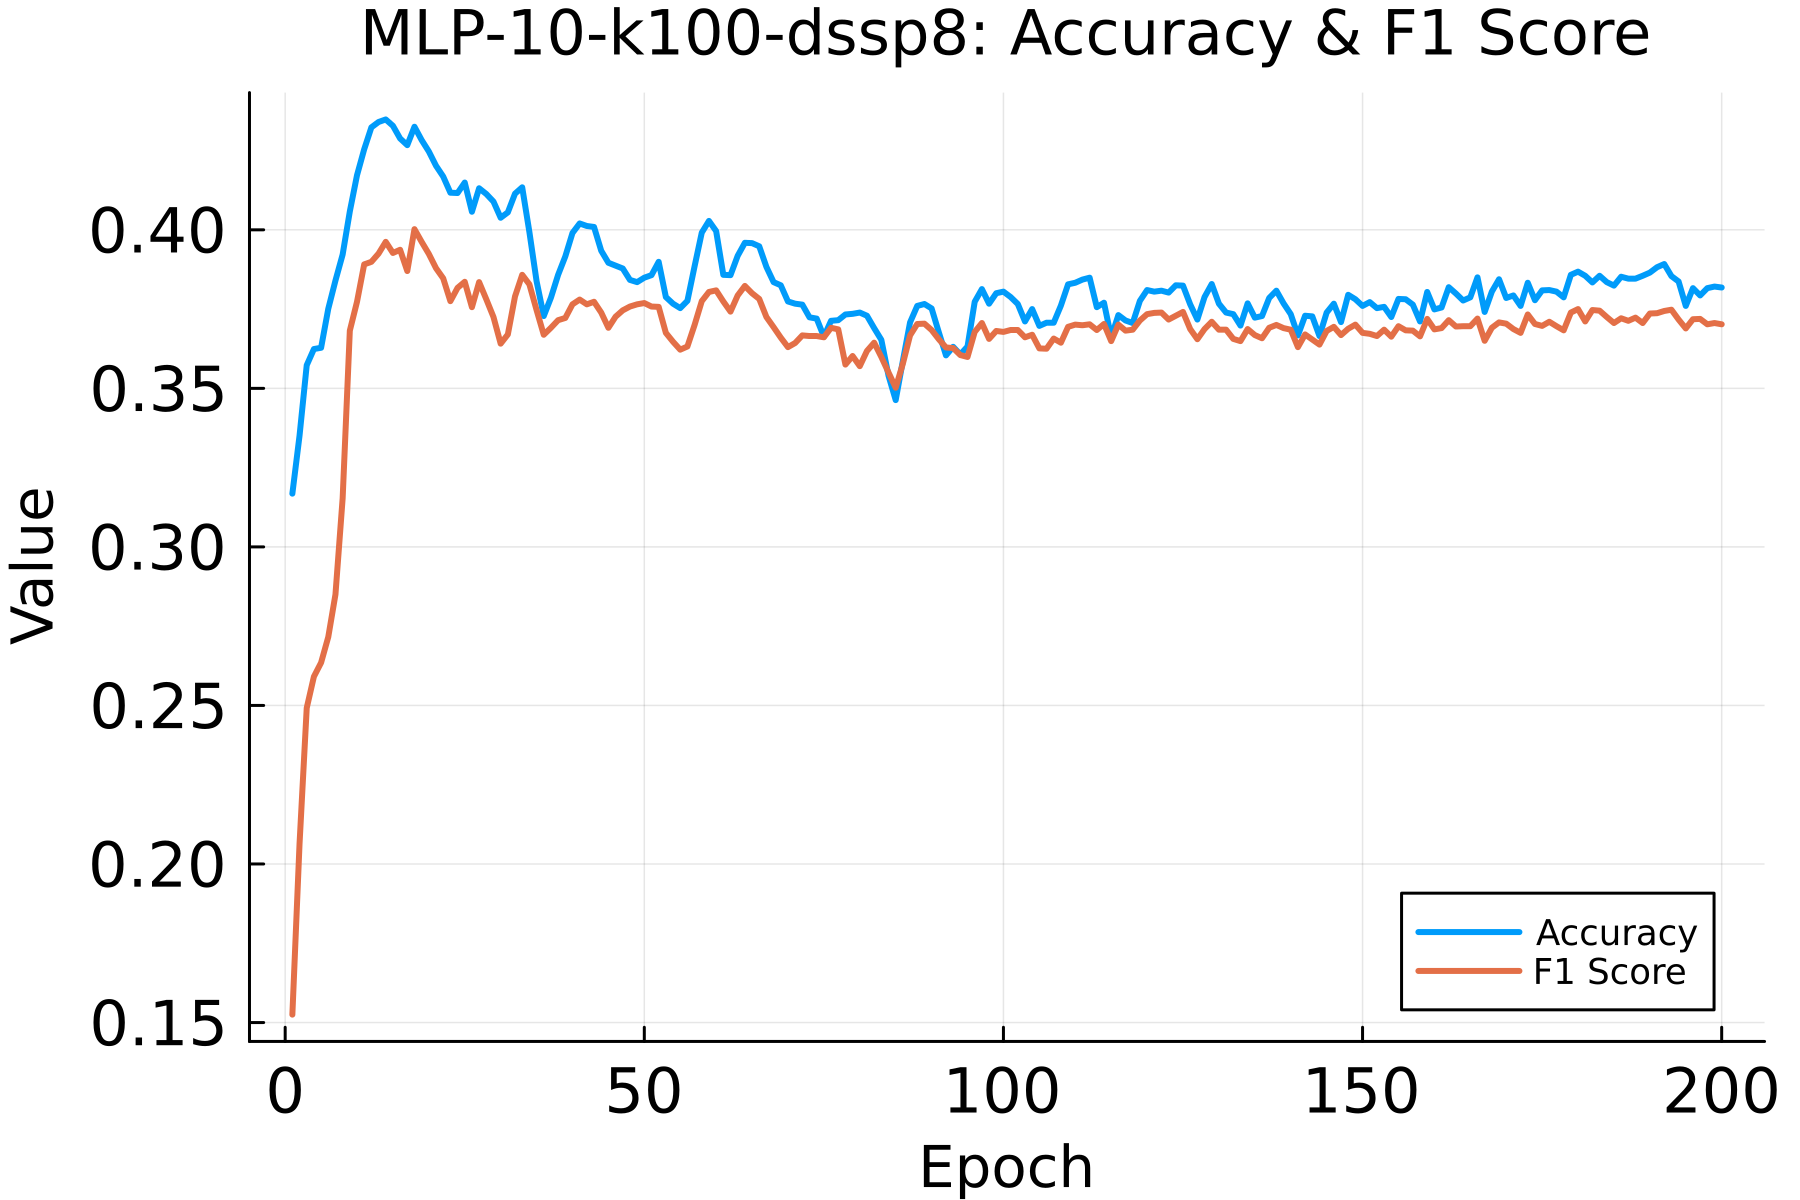
\includegraphics[width=\textwidth]{mlpfull_k100_dssp8_score}
        \label{fig:she}
    \end{subfigure}
    \caption{Performance of training procedure of the 10-layer MLP model on 60 \% of NetSurfP 2.0's training data, 0.8-0.2 training-test data split. Tested on 3 and 8 secondary structure classifications (dssp3 and dssp8 respectively) and with different kinds of hyperdimensional embeddings made with neighborhood-encoding ($n = 25$ and $n=100$).}
    \label{fig:main8e}
  \end{figure}

The fully trained 10-layer MLP models were evaluated on the test datasets with the results summarized in table~\ref{tab:casp} and table~\ref{tab:casp2}. To validate our findings, we also generated a randomly generated dataset for comparison. Disappointingly, the model's performance on the test data did not surpass its own performance on the randomly generated data, meaning that our model is not able to accurately predict the secondary structure of an amino acid based on its neighborhood-encoding.

\begin{table}[h]
    \caption{Accuracies of secondary structure classification of a 10-layer MLP model trained on 60 \% of NetSurfP 2.0's training data encoded into different kinds of hyperdimensional embeddings made with neighborhood-encoding ($n = 25$ and $n=100$). Tested on the CASP12 and CB513 dataset. Performance with randomly generated data was also assessed.}
    \label{tab:casp}
    \centering
    \begin{tabular}{l|cc|cc|cc}
        \toprule
        \textbf{Accuracy} & \multicolumn{2}{c|}{CASP12} & \multicolumn{2}{c|}{CB513} & \multicolumn{2}{c|}{Random}\\
        & ss3 & ss8 & ss3 & ss8 & ss3 & ss8\\
        \midrule
        \textbf{n25} & 36.9 & 24.88 & 35.48 & 21.01 & 34.11 & 21.09 \\
        \textbf{n100} & 39.33 & 23.13 & 37.61 & 20.86 & 38.74 & 20.53\\
        \bottomrule
    \end{tabular}
\end{table}

\begin{table}[h]
    \caption{F1-scores of secondary structure classification of a 10-layer MLP model trained on 60 \% of NetSurfP 2.0's training data encoded into different kinds of hyperdimensional embeddings made with neighborhood-encoding ($n = 25$ and $n=100$). Tested on the CASP12 and CB513 dataset. Performance with randomly generated data was also assessed.}
    \label{tab:casp2}
    \centering
    \begin{tabular}{l|cc|cc|cc}
        \toprule
        \textbf{F1} & \multicolumn{2}{c|}{CASP12} & \multicolumn{2}{c|}{CB513} & \multicolumn{2}{c}{Random}\\
        & ss3 & ss8 & ss3 & ss8 & ss3 & ss8 \\
        \midrule
        \textbf{n25} & 37.50 & 18.61 & 35.52 & 15.30 & 34.35 & 14.79\\
        \textbf{n100} & 37.19 & 20.25 & 35.68 & 18.03 & 36.07 & 17.80\\
        \bottomrule
    \end{tabular}
\end{table}

\section{Discussion}
Our exploration into the use of various perceptron-based neural network models for protein secondary structure prediction has yielded several insights. The overarching observation from our results is that our models have not effectively learned from the data. This suggests a couple of potential areas for improvement.

Firstly, the relative simplicity of our neural network models may be a limiting factor. The high-dimensional sparse vectors that represent our data may require a more complex model to capture the intricate patterns within the data effectively. This could involve exploring more sophisticated architectures, such as deeper networks or alternative architectures. A hyperdimensional computing-based method such as OnlineHD might be an interesting learning method too for later research.

Secondly, the neighborhood-encoding algorithm we employed may require further refinement. The quality of the embeddings produced by this algorithm directly impacts the ability of the model to learn. Optimizing this algorithm to produce more informative or discriminative embeddings could potentially enhance the learning capability of our models. As said earlier, there might be a case of oversaturation in the vectors and therefore a loss of information on the complex intricacies in the data since binary vectors were used to encode the data. Interesting avenues might include using real-valued vectors to generate neighborhood-encodings. This algorithm could be coupled with weighted additions to avoid oversaturation of vectors.

Lastly, the size of the training dataset could also be a contributing factor. Given the computational constraints of this study, we were limited in the amount of data we could use for training. However, machine learning models, especially deep neural networks, often benefit from larger datasets. Increasing the size of the training dataset could provide our models with more examples to learn from, potentially improving their performance.

In order to benchmark our study against the capabilities of state-of-the-art protein language models, we collected the available results of other protein language models on similar experiments. The models include ESM-1b~\cite{esm}, NetSurfP 2.0~\cite{netsurf}, its successor NetSurfP 3.0~\cite{netsurf3} and ProtTrans' best-performing model; ProtT5-XL-U50~\cite{prottrans}. ESM-1b is a model by Meta AI, trained on a large corpus of approximately 86 billion amino acid residues. It consists of around 670 million parameters and utilizes a transformer architecture together with evolutionary data. NetsurfP 2.0 and its successor NetSurf 3.0 are models comprising convolutional neural network (CNN) and bidirectional long short-term (biLSTM) layers. Despite not relying on a transformer-based architecture and having been trained on a comparatively smaller dataset, they exhibit state-of-the-art performance. The distinction between these two methods lies in their input configurations. ProtT5-XL-U50 is a large transformer-based model comprising 3 billion parameters, trained on UniRef50 which comprises roughly 45 million sequences~\cite{uniref}.

\begin{table}[h]
    \caption{Accuracies of secondary structure classification of state-of-the-art protein language models. Tested on 3 and 8 secondary structure classifications of the CASP12 and CB513 dataset.}
    \label{tab:casp3}
    \centering
    \begin{tabular}{lcc|cc}
        \toprule
        \textbf{Accuracy} & \multicolumn{2}{c|}{CASP12} & \multicolumn{2}{c|}{CB513}\\
        & ss3 & ss8 & ss3 & ss8\\
        \midrule
        \textbf{ESM-1b} & 76.9 & 83.9 & 66.0 & 70.2\\
        \textbf{NetSurfP 2.0} & 82.0 & 84.5 & 66.9 & 71.3\\
        \textbf{NetSurfP 3.0} & 79.1 & 84.5 & 66.9 & 71.1\\
        \textbf{ProtT5-XL-U50} & 77.5 & 86.2 & 70.5 & 74.5\\
        \bottomrule
    \end{tabular}
  \end{table}

  When compared to the performance of state-of-the-art protein language models in table~\ref{tab:casp3}, our models fall short in performance. This underscores the complexity of protein secondary structure prediction and the need for models that can effectively learn from the intricate patterns in the data.
